


% \begin{table*}[t]
% \centering
% \caption{Comparison with other state-of-the-art real-time object detectors on MS COCO dataset.}
%   \label{tab:coco_compare}
% \renewcommand{\arraystretch}{1.0}
% \begin{tabular}{lcccccc}
% \toprule
% Method & FLOPs (G) & Param.(M) & $\text{AP}_{50:95}^\text{val}$ & $\text{AP}_{50}^\text{val}$ & $\text{AP}_{75}^\text{val}$ & Latency (ms) \\
% \midrule
% YOLOv6-3.0-N        & 11.4  & 4.7  & 37.0  & 52.7  & –    & 2.7 \\
% Gold-YOLO-N         & 12.1  & 5.6  & 39.6  & 55.7  & –    & 2.9 \\
% YOLOv8-N            & 8.7   & 3.2  & 37.4  & 52.6  & 40.5 & 1.8 \\
% YOLOv10-N& –     & –    & –     & –     & –    & –   \\
% YOLO11-N& 6.5   & 2.6  & 38.6  & 54.2  & 41.6 & –   \\
% YOLOv12-N& 6.5   & 2.6  & 40.1  & 56.0  & 43.4 & –   \\
% YOLOv13-Nano        & 6.4   & 2.5  & 41.6(+1.5) & 57.8(+1.8) & 45.1 & –   \\
% \midrule
% YOLOv6-3.0-S        & 45.3  & 18.5 & 44.3  & 61.2  & –    & 3.4 \\
% Gold-YOLO-S         & 46.0  & 21.5 & 45.4  & 62.5  & –    & 3.8 \\
% YOLOv8-S            & 28.6  & 11.2 & 45.0  & 61.8  & 48.7 & 2.3 \\
% RT-DETR-R18         & 60.0  & 20.0 & 46.5  & 63.8  & –    & 4.6 \\
% RT-DETRv2-R18       & 60.0  & 20.0 & 47.9  & 64.9  & –    & 4.6 \\
% YOLOv9-S            & 26.4  & 7.1  & 46.8  & 63.4  & 50.7 & –   \\
% YOLOv10-S           & 21.6  & 7.2  & 46.3  & 63.0  & 50.4 & 2.5 \\
% YOLOv10-S& 21.6  & 7.2  & 45.6  & 62.6  & 49.4 & –   \\
% YOLO11-S& 21.5  & 9.4  & 45.8  & 62.6  & 49.8 & –   \\
% YOLOv12-S& 21.4  & 9.3  & 47.1  & 64.2  & 51.0 & –   \\
% YOLOv13-Small       & 20.8  & 9.0  & 48.0(+0.9) & 65.2(+1.0) & 52.0 & –   \\
% \midrule
% YOLOv6-3.0-L        & 150.7 & 59.6 & 51.8  & 69.2  & –    & 9.0 \\
% Gold-YOLO-L         & 151.7 & 75.1 & 51.8  & 68.9  & –    & 10.7 \\
% YOLOv8-L            & 165.2 & 43.7 & 53.0  & 69.8  & 57.7 & 8.1 \\
% RT-DETR-R50         & 136.0 & 42.0 & 53.1  & 71.3  & –    & 6.9 \\
% RT-DETRv2-R50       & 136.0 & 42.0 & 53.4  & 71.6  & –    & 6.9 \\
% YOLOv9-C            & 102.1 & 25.3 & 53.0  & 70.2  & 57.8 & –   \\
% YOLOv10-B           & 92.0  & 19.1 & 52.5  & 69.6  & 57.2 & 5.7 \\
% YOLOv10-L           & 120.3 & 24.4 & 53.2  & 70.1  & 58.1 & 7.3 \\
% YOLOv10-L& –     & –    & –     & –     & –    & –   \\
% YOLO11-L& 86.9  & 25.3 & 51.3  & 68.2  & 55.7 & –   \\
% YOLOv12-L& 88.9  & 26.4 & 53.0  & 70.0  & 57.9 & –   \\
% YOLOv13-Plus        & 88.4  & 27.6 & 53.4  & 70.9  & 58.1 & –   \\
% \midrule
% YOLOv8-X            & 257.8 & 68.2 & 54.0  & 71.0  & 58.8 & 12.8 \\
% RT-DETR-R101        & 259.0 & 76.0 & 54.3  & 72.7  & –    & 13.5 \\
% RT-DETRv2-R101      & 259.0 & 76.0 & 54.3  & 72.8  & –    & 13.5 \\
% YOLOv10-X& –     & –    & –     & –     & –    & –   \\
% YOLO11-X& –     & –    & –     & –     & –    & –   \\
% YOLOv12-X& –     & –    & –     & –     & –    & –   \\
% YOLOv13-Ultra       & 199.2 & 64.0 & 54.8  & 72.0  & 59.8 & –   \\
% \bottomrule
% \end{tabular}
% \end{table*}

\begin{table*}[t]
\centering
\caption{Quantitative comparison with other state-of-the-art real-time object detectors on MS COCO dataset.}
\vspace{-0.2cm}
\label{tab:coco_compare}
\renewcommand{\arraystretch}{1.}
\setlength{\tabcolsep}{5.8mm}
\begin{tabular}{lcccccc}
\toprule
\textbf{Method} & \textbf{FLOPs (G)} & \textbf{Parameters (M)} & \textbf{$\text{AP}_{50:95}^\text{val}$} & \textbf{$\text{AP}_{50}^\text{val}$} & \textbf{$\text{AP}_{75}^\text{val}$} & \textbf{Latency (ms)} \\ \midrule
YOLOv6-3.0-N~\cite{yolov6}        & 11.4  & 4.7  & 37.0  & 52.7  & –    & 2.74\\
Gold-YOLO-N~\cite{goldyolo}        & 12.1  & 5.6  & 39.6  & 55.7  & –    & 2.97\\
YOLOv8-N~\cite{yolov8}            & 8.7   & 3.2  & 37.4  & 52.6  & 40.5 & 1.77\\
YOLOv10-N~\cite{yolov10}           & 6.7& 2.3& 38.5& 53.8& 41.7& 1.84\\
YOLO11-N~\cite{yolo11}            & 6.5   & 2.6  & 38.6  & 54.2  & 41.6 & 1.53\\
YOLOv12-N~\cite{yolov12}           & 6.5   & 2.6  & 40.1  & 56.0  & 43.4 & 1.83\\\rowcolor{blue!10}
\textbf{YOLOv13-N}& \textbf{6.4}   & \textbf{2.5}  & \textbf{41.6} & \textbf{57.8} & \textbf{45.1} & \textbf{1.97}\\ \midrule
YOLOv6-3.0-S~\cite{yolov6}        & 45.3  & 18.5 & 44.3  & 61.2  & –    & 3.42\\
Gold-YOLO-S~\cite{goldyolo} & 46.0  & 21.5 & 45.4  & 62.5  & –    & 3.82\\
YOLOv8-S~\cite{yolov8}            & 28.6  & 11.2 & 45.0  & 61.8  & 48.7 & 2.33\\
RT-DETR-R18~\cite{rt_detr}         & 60.0  & 20.0 & 46.5  & 63.8  & –    & 4.58\\
RT-DETRv2-R18~\cite{rt_detrv2}       & 60.0  & 20.0 & 47.9  & 64.9  & –    & 4.58\\
YOLOv9-S~\cite{yolov9}            & 26.4  & 7.1  & 46.8  & 63.4  & 50.7 & 3.44\\
YOLOv10-S~\cite{yolov10}           & 21.6  & 7.2  & 46.3& 63.0& 50.4& 2.53\\
YOLO11-S~\cite{yolo11}            & 21.5  & 9.4  & 45.8  & 62.6  & 49.8 & 2.56\\
YOLOv12-S~\cite{yolov12}           & 21.4  & 9.3  & 47.1  & 64.2  & 51.0 & 2.82\\ \rowcolor{blue!10}
\textbf{YOLOv13-S}& \textbf{20.8}  & \textbf{9.0}  & \textbf{48.0} & \textbf{65.2} & \textbf{52.0} & \textbf{2.98}\\ \midrule
YOLOv6-3.0-L~\cite{yolov6}        & 150.7 & 59.6 & 51.8  & 69.2  & –    & 9.01\\
Gold-YOLO-L~\cite{goldyolo}         & 151.7 & 75.1 & 51.8  & 68.9  & –    & 10.69\\
YOLOv8-L~\cite{yolov8}            & 165.2 & 43.7 & 53.0  & 69.8  & 57.7 & 8.13\\
RT-DETR-R50~\cite{rt_detr}         & 136.0 & 42.0 & 53.1  & 71.3  & –    & 6.93\\
RT-DETRv2-R50~\cite{rt_detrv2}       & 136.0 & 42.0 & 53.4  & 71.6  & –    & 6.93\\
YOLOv9-C~\cite{yolov9}            & 102.1 & 25.3 & 53.0  & 70.2  & 57.8 & 6.64\\
YOLOv10-L~\cite{yolov10}           & 120.3& 24.4& 53.2& 70.1& 57.2& 7.31\\
YOLO11-L~\cite{yolo11}            & 86.9  & 25.3 & 52.3& 69.2& 55.7 & 6.23\\
YOLOv12-L~\cite{yolov12}           & 88.9  & 26.4 & 53.0  & 70.0  & 57.9 & 7.10\\ \rowcolor{blue!10}
\textbf{YOLOv13-L}& \textbf{88.4}  & \textbf{27.6} & \textbf{53.4}  & \textbf{70.9}  & \textbf{58.1} & \textbf{8.63}\\ \midrule
YOLOv8-X~\cite{yolov8}            & 257.8 & 68.2 & 54.0  & 71.0  & 58.8 & 12.83\\
RT-DETR-R101~\cite{rt_detr}        & 259.0 & 76.0 & 54.3  & 72.7  & –    & 13.51\\
RT-DETRv2-R101~\cite{rt_detrv2}      & 259.0 & 76.0 & 54.3  & 72.8  & –    & 13.51\\
YOLOv10-X~\cite{yolov10}           & 160.4     & 29.5    & 54.4& 71.3& 59.3& 10.70\\
YOLO11-X~\cite{yolo11}            & 194.9& 56.9& 54.2& 71.0& 59.1& 11.35\\
YOLOv12-X~\cite{yolov12}           & 199.0     & 59.1    & 54.4    & 71.1& 59.3& 12.46\\ \rowcolor{blue!10}
\textbf{YOLOv13-X}& \textbf{199.2} & \textbf{64.0} & \textbf{54.8}  & \textbf{72.0}  & \textbf{59.8} & \textbf{14.67}\\
\bottomrule
\end{tabular}
\vspace{-0.4cm}
\end{table*}



\section{Experiments}
To validate the effectiveness and efficiency of our proposed YOLOv13 model, we conduct extensive experiments. In Sec.~\ref{sec:setting}, we introduce the detailed experimental settings. Then, in Sec.~\ref{sec:cmp}, we compare our proposed method with other existing real-time object detection methods to demonstrate the validity of our method. Finally, we conduct ablation experiments in Sec.~\ref{sec:ablation} to prove the effectiveness of each proposed module.

\subsection{Experimental Setting}
\label{sec:setting}
 
\subsubsection{Dataset}
We use the Microsoft COCO (MS COCO) dataset~\cite{mscoco}, the most widely adopted benchmark for the object detection task, to evaluate our YOLOv13 model and other state‐of‐the‐art real‐time detectors. The MS COCO dataset training set (Train2017) contains approximately 118,000 images, and the validation set (Val2017) contains approximately 5,000 images, covering 80 common object categories in natural scenes. In our implementation, all methods are trained on the Train2017 subset and tested on the Val2017 subset.

As the YOLO series continues to evolve, models with greater generality and stronger generalization capabilities become increasingly important. To this end, we include cross-domain generalization under distribution shifts in our evaluation. As a supplementary benchmark, we select the Pascal VOC 2007 dataset~\cite{voc}, which contains a combined total of 5,011 images in the training and validation sets and 4,952 images in the test set, covering 20 common object classes. To evaluate the cross-domain generalization ability, all methods are directly evaluated on the Pascal VOC 2007 test set using the model trained on the MS COCO dataset.


\subsubsection{Implementation Details}
Similar to previous YOLO models, our YOLOv13 family includes four variants: Nano (N), Small (S), Large (L), and Extra-Large (X). For the N, S, L, and X models, the number of hyperedges $M$ is set to 4, 8, 8, and 12, respectively. For all variants, we train the model for 600 epochs with a batch size of 256. The initial learning rate is 0.01 and SGD is used as the optimizer, which is consistent with YOLO11 and YOLOv12 models. A linear decay scheduler is adopted, and a linear warm‐up is applied within the first 3 epochs. During training, the input image size is set to \(640 \times 640\). We employ the same data augmentation techniques as previous YOLO versions, including Mosaic and Mixup. 
% We use 4 and 8 RTX 4090 GPUs to train YOLOv13‐N and YOLOv13‐S, use 4 and 8 A800 GPUs to train YOLOv13‐P and YOLOv13‐U, respectively. 
We use 4 and 8 RTX 4090 GPUs to train YOLOv13-N and YOLOv13-S, respectively, and use 4 and 8 A800 GPUs to train YOLOv13-L and YOLOv13-X, respectively.
Additionally, following the standard practice of previous YOLO series, we evaluate the latency on a single Tesla T4 GPU using TensorRT FP16 for all models. 
In addition, it should be noted that, to ensure fair and rigorous comparison, we reproduce all variants of the previous YOLO11 and YOLOv12 (v1.0 version) models using their official settings on the same hardware platform as our YOLOv13 model.


\subsection{Comparison with Other Methods}
\label{sec:cmp}
Table~\ref{tab:coco_compare} shows the quantitative comparison results on the MS COCO dataset. Our proposed method is compared with previous YOLO series models. As mentioned above, our YOLOv13 model and the latest YOLO11 and YOLOv12 models are trained on the same GPUs while the existing methods are trained using their official code and training parameters. From the table, we can observe that all variants of our YOLOv13 model achieve state-of-the-art performance while remaining lightweight. Specifically, compared with the previous YOLOv12 model, our YOLOv13 model can improve $\text{AP}_{50:95}^\text{val}$ by 1.5\%, 0.9\%, 0.4\%, and 0.4\%, and improve $\text{AP}_{50}^\text{val}$ by 1.8\%, 1.0\%, 0.9\%, and 0.9\% in terms of Nano, Small, Large, and Extra-Large models, respectively. In addition, compared with ViT-based methods, our proposed YOLOv13 model can also achieve better detection accuracy with fewer parameters and lower computational complexity. Compared to RT-DETRv2-R18, our YOLOv13-S model can improve $\text{AP}_{50:95}^\text{val}$ by 0.1\% while reducing the number of parameters by 55.0\% and the FLOPs by 65.3\%. Furthermore, from the table, we can observe that our proposed method can achieve more significant advantages in lightweight variants, \eg, the Nano model. This is also the core objective of the YOLO series of models, \ie, more accurate, faster, and lighter. This is because our proposed core HyperACE mechanism can more fully explore the multi-to-multi correlations in complex scenarios. As the high-order version of the traditional self-attention mechanism, HyperACE leverages high-order correlations as guidance to achieve accurate feature enhancement with low parameter counts and computational complexity. These quantitative comparison results prove the effectiveness of our proposed YOLOv13 model.
\begin{figure*}
    \centering
    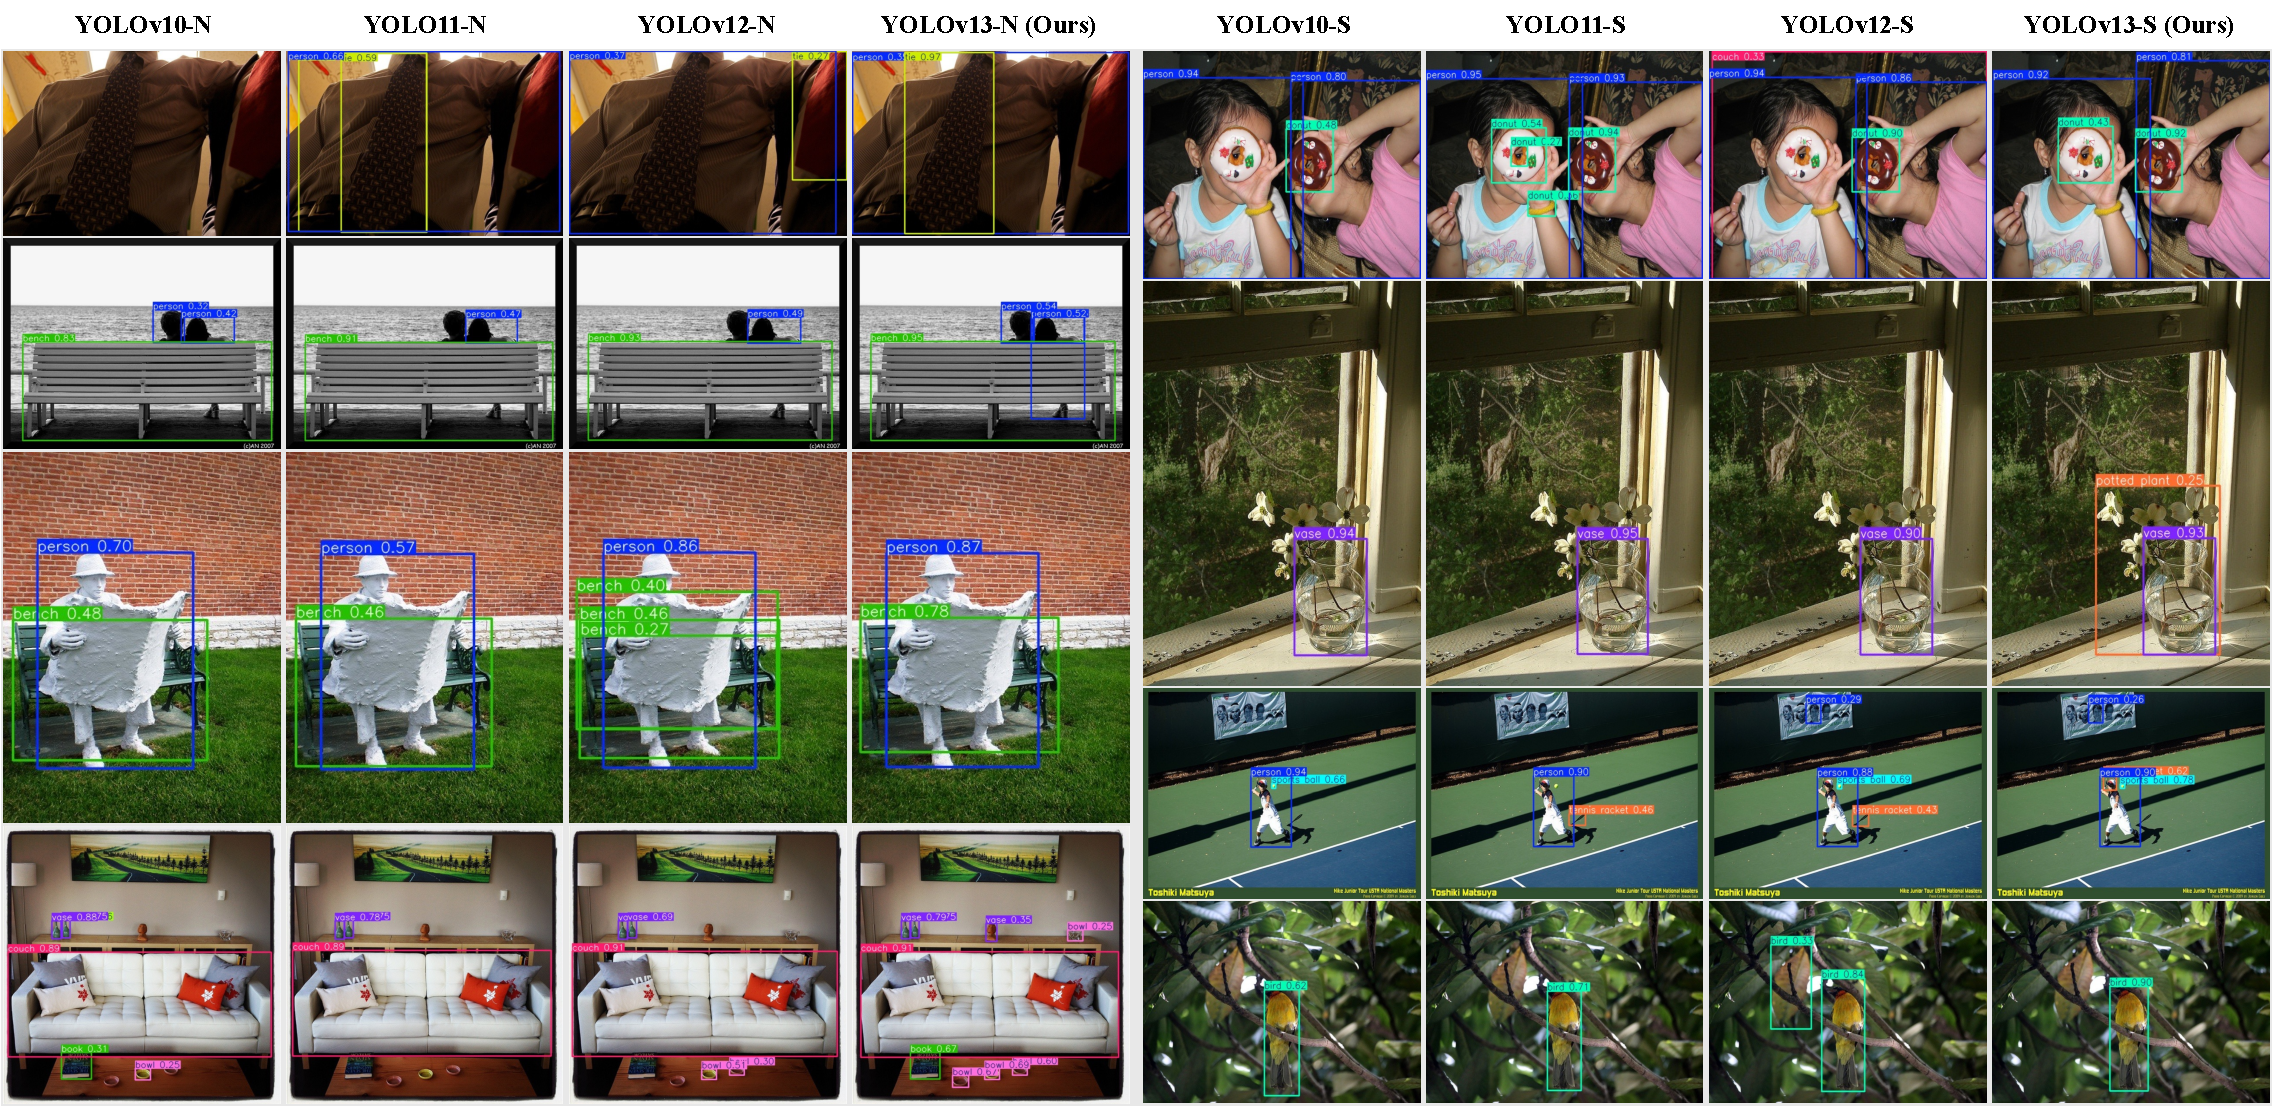
\includegraphics[width=1\linewidth]{figures/vis_bbox.pdf}
    \vspace{-0.5cm}
    \caption{Qualitative comparison on MS COCO dataset~\cite{mscoco}. From left to right: detection results generated from YOLOv10-N/S~\cite{yolov10}, YOLO11-N/S~\cite{yolo11}, YOLOv12-N/S~\cite{yolov12}, and our YOLOv13-N/S models, respectively. Our method can achieve better detection performance in complex scenes. 
    % Best viewed in color.
    }
    \vspace{-0.5cm}
    \label{fig:vis_bbox}
\end{figure*}

\begin{table}[!tp]
\centering
\caption{Generalizability comparison of our method with other real-time object detectors. All models are trained on MS COCO dataset and tested on Pascal VOC 2007 dataset.}
\label{tab:voc_compare}
\renewcommand{\arraystretch}{1.15}
\setlength{\tabcolsep}{5.6mm}
\begin{tabular}{lccc}
\toprule
\textbf{Method} & \textbf{$\text{AP}_{50:95}^\text{val}$} & \textbf{$\text{AP}_{50}^\text{val}$} & \textbf{$\text{AP}_{75}^\text{val}$} \\
\midrule
YOLOv8-N~\cite{yolov8}            & 60.4& 80.4& 67.1\\
YOLOv10-N~\cite{yolov10}           & 61.8& 81.0& 68.3\\
YOLO11-N~\cite{yolo11}            & 62.1& 81.5& 68.9\\
YOLOv12-N~\cite{yolov12}           & 64.3& 83.0& 71.2\\
\rowcolor{blue!10}
\textbf{YOLOv13-N}        & \textbf{65.3}& \textbf{83.3}& \textbf{72.4}\\
\midrule
YOLOv8-S~\cite{yolov8}            & 66.4& 84.6& 72.4\\
YOLOv9-S~\cite{yolov9}            & 68.9& 85.8& 74.0\\
YOLOv10-S~\cite{yolov10}           & 67.7& 85.0& 75.9\\
YOLO11-S~\cite{yolo11}            & 67.7& 85.2& 74.8\\
YOLOv12-S~\cite{yolov12}           & 69.7& 86.5& 77.2\\
\rowcolor{blue!10}
\textbf{YOLOv13-S}       & \textbf{70.1} & \textbf{86.7}& \textbf{77.4}\\
\bottomrule
\end{tabular}
\vspace{-0.5cm}
\end{table}


% qualitative
Figure~\ref{fig:vis_bbox} shows the qualitative comparison results on the MS COCO dataset. Our proposed YOLOv13 model is compared with the existing YOLOv10~\cite{yolov10}, YOLO11~\cite{yolo11}, and YOLOv12~\cite{yolov12} models. From the figure, we can observe that our YOLOv13 model can achieve more accurate detection performance in complex scenes. Specifically, as shown in the last row on the left side of Fig.~\ref{fig:vis_bbox}, our YOLOv13-N model can accurately detect objects in complex multi-object scenes. In contrast, previous models miss small objects such as bowls and vases. This is due to the fact that our proposed HyperACE can establish high-order correlations between multiple related objects, enabling accurate detection of multiple targets in complex scenes. As shown in the second row on the right side, only our method successfully detects the plant behind the vase, which is a challenging scenario. Intuitively, the vase and the plant are strongly associated, leading to a high probability appearance of the plant. Our method can achieve accurate detection by mining such latent correlations. As shown in the third row on the right side, our method can accurately detect the tennis racket held by the athlete, while previous methods either missed it or incorrectly detected the shadow. These qualitative results demonstrate the effectiveness of our proposed method.


% generalization ability
As mentioned above, to validate the generalization ability of our proposed method, we train our YOLOv13 model and previous YOLO models on the MS COCO dataset and test all methods on the Pascal VOC 2007 dataset. The quantitative results are shown in Tab.~\ref{tab:voc_compare}. From the table, we can observe that our proposed YOLOv13 model achieves satisfactory generalization performance. Specifically, compared to the previous YOLOv12 model, our proposed method improves the $\text{AP}_{50:95}^\text{val}$ by 1.0\% and 0.4\% in terms of Nano and Small models, respectively. More significant performance improvements can be achieved compared to earlier models. These results demonstrate the generalization ability of our proposed method.



\subsection{Ablation Study}
\label{sec:ablation}
\subsubsection{FullPAD and HyperACE} To validate the effectiveness and necessity of our proposed FullPAD paradigm and HyperACE mechanism, we evaluate the performance of the proposed YOLOv13-Small model when FullPAD distributes the features to different locations. The quantitative results are shown in Tab.~\ref{tab:distribution}. Specifically, when FullPAD does not distribute any features, it is equivalent to removing the proposed HyperACE, and the results under such setting are shown in the first row of the table. From the table, we can observe that the removal of the proposed HyperACE will reduce the $\text{AP}_{50:95}^\text{val}$ and $\text{AP}_{50}^\text{val}$ by 0.9\% and 1.1\%, respectively. This result demonstrates the effectiveness of adaptive correlation enhancement. In addition, when FullPAD distributes enhanced features only to the backbone-neck (left FullPAD tunnel in Fig.~\ref{fig:framework}), in-neck (middle FullPAD tunnel in Fig.~\ref{fig:framework}), and neck-head (right FullPAD tunnel in Fig.~\ref{fig:framework}), the $\text{AP}_{50:95}^\text{val}$ will decrease by 0.2\%, 0.4\%, and 0.3\%, respectively, compared to the full model. These results demonstrate the necessity of our proposed FullPAD paradigm.

\begin{table}[!tp]
\centering
\setlength{\tabcolsep}{2.8mm}
\caption{Impact of setting different FullPAD distribution locations on the performance of our YOLOv13-S model.}
\vspace{-0.1cm}
\label{tab:distribution}
\renewcommand{\arraystretch}{1.0}
\begin{tabular}{ccccc}
\toprule
\textbf{Backbone-Neck} & \textbf{In-Neck} & \textbf{Neck-Head} & \textbf{$\text{AP}_{50:95}^\text{val}$} & \textbf{$\text{AP}_{50}^\text{val}$} \\
\midrule
\ding{56}  & \ding{56} & \ding{56} & 47.1& 64.1\\
\ding{52}  & \ding{56} & \ding{56} & 47.8& 65.0\\
\ding{56}  & \ding{52} & \ding{56} & 47.6& 64.8\\
\ding{56} & \ding{56} & \ding{52} & 47.7& 64.9\\
\ding{52} & \ding{52} & \ding{52} & 48.0& 65.2\\
\bottomrule
\end{tabular}
\vspace{-0.4cm}
\end{table}

\begin{table}[!tp]
\centering
\setlength{\tabcolsep}{2.6mm}
\caption{Impact of different numbers of hyperedges ($M$) on the performance of our YOLOv13-S model.}
\vspace{-0.1cm}
\label{tab:num_edge}
\renewcommand{\arraystretch}{1.0}
\begin{tabular}{cccccc}
\toprule
$M$ & \textbf{FLOPs (G)} & \textbf{Param. (M)} & \textbf{$\text{AP}_{50:95}^\text{val}$} & \textbf{$\text{AP}_{50}^\text{val}$} & \textbf{$\text{AP}_{75}^\text{val}$} \\
\midrule

2  & 20.4 & 8.6 & 47.8 & 64.7 & 51.9 \\
4  & 20.5& 8.8& 47.9& 65.0& 51.9\\
8  & 20.8 & 9.0 & 48.0 & 65.2 & 52.0 \\
16 & 21.5  & 9.6 &  48.1  & 65.2     &  52.1      \\
\bottomrule
\end{tabular}
\vspace{-0.4cm}
\end{table}

\begin{table}[!tp]
\centering
\setlength{\tabcolsep}{1.2mm}
\caption{Impact of the DS blocks on the performance of our YOLOv13 Nano and Small models.}
\vspace{-0.1cm}
\label{tab:dsblocks}
\renewcommand{\arraystretch}{1.0}
\begin{tabular}{lccccc}
\toprule
\textbf{Method} & \textbf{DS Blocks} & \textbf{FLOPs (G)} & \textbf{Param. (M)} & \textbf{$\text{AP}_{50:95}^\text{val}$} & \textbf{$\text{AP}_{50}^\text{val}$} \\ \midrule
YOLOv13-N& \ding{52}  & 6.4  & 2.5  & 41.6 & 57.8 \\
YOLOv13-N& \ding{56}  & 7.9  & 3.1  & 41.6 & 57.9 \\ \midrule
YOLOv13-S& \ding{52}  & 20.8 & 9.0  & 48.0 & 65.2 \\
YOLOv13-S& \ding{56}  & 27.1 & 11.7 & 48.0 & 65.3 \\
\bottomrule
\end{tabular}
\vspace{-0.3cm}
\end{table}



% Adaptive correlation modeling
Figure~\ref{fig:vis_soft} shows the visualization of representative hyperedges generated by adaptive hypergraph construction in the proposed HyperACE module. From the figure, we can intuitively observe the high-order visual correlations captured by the proposed HyperACE, which helps to enhance the interpretability of the model. As shown in the first and second column of the figure, HyperACE can effectively model the correlations among multiple foreground objects or partial elements within a scene, \eg, the skis and skistick in the first row, and the cars and multiple traffic lights in the second row. As shown in the third column, our proposed method can also model the correlations between foreground objects and the background scene, \eg, the tennis racket and tennis court in the third row, and the baseball glove and the baseball field in the last row. These visualizations demonstrate the modeling capabilities of our proposed HyperACE module for potential high-order correlations within scenes, enabling the model to enhance features based on multi-to-multi correlations rather than just low-order pairwise correlations.
\begin{figure}
    \centering
    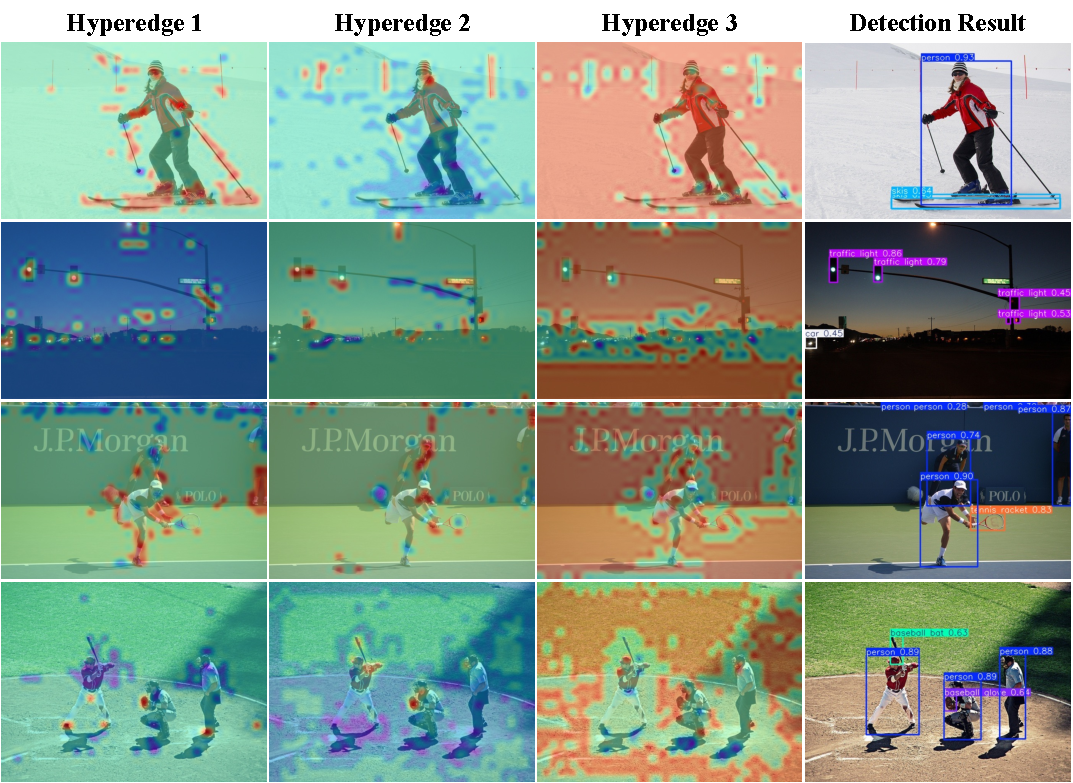
\includegraphics[width=1\linewidth]{figures/vis_edge.pdf}
    \vspace{-0.6cm}
    \caption{Visualization of adaptive hyperedges. The hyperedges in the first and second columns mainly focus on the high-order interactions among objects in the foreground. The third column mainly focuses on the interactions between the background and the foreground targets. The visualization of these adaptive hyperedges can intuitively reflect the high-order visual correlations modeled by our YOLOv13.}
    \vspace{-0.5cm}
    \label{fig:vis_soft}
\end{figure}

\begin{table}[!tp]
\centering
\setlength{\tabcolsep}{2.6mm}
\caption{Impact of different training epochs on the performance of our YOLOv13 Nano and Small models.}
\label{tab:epoch}
\renewcommand{\arraystretch}{1.0}
\begin{tabular}{lcccc}
\toprule
\textbf{Epochs} & \textbf{$\text{AP}_{50:95}^\text{val}$ (N)} & \textbf{$\text{AP}_{50}^\text{val}$ (N)} & \textbf{$\text{AP}_{50:95}^\text{val}$ (S)} & \textbf{$\text{AP}_{50}^\text{val}$ (S)} \\
\midrule
300  & 39.5& 55.2& 46.9& 63.1\\
500  & 41.4& 57.6& 47.8& 64.9\\
600  & 41.6& 57.8& 48.0& 65.2\\
800 & 41.3& 57.3& 47.8& 64.7\\
\bottomrule
\end{tabular}
\vspace{-0.4cm}
\end{table}
\begin{table}[!tp]
\centering

\setlength{\tabcolsep}{3.8mm}
\caption{Inference latency (ms) for FP16 precision on various computing devices. }
\vspace{-0.2cm}
\label{tab:latency}
\renewcommand{\arraystretch}{1.0}
\begin{tabular}{lccc}
\toprule
\textbf{Method}           & \textbf{Tesla T4} & \textbf{RTX 4090} & \textbf{CPU (ONNX)}\\
\midrule
YOLOv13-N     & 1.97& 1.25& 39.97\\
YOLOv13-S    & 2.98& 1.27& 61.12\\
YOLOv13-L     & 8.63& 2.36& 185.36\\
YOLOv13-X    & 14.67& 3.10& 330.12\\
\bottomrule
\end{tabular}
\vspace{-0.3cm}
\end{table}

% Xeon R Platinum

\subsubsection{Number of hyperedges} To validate the effect of the number of hyperedges $M$ on model performance, we set different numbers of hyperedges and test the performance of the YOLOv13-S model. Table~\ref{tab:num_edge} shows the quantitative results. From the table, we can observe that fewer hyperedges result in fewer model parameters and less computational effort, but also lead to a decline in performance. This is due to insufficient correlation modeling of the scene. When the number of hyperedges is increased to 16, the detection performance still improves, but it also brings additional parameters and computational costs. Similar results can be observed for other model variants. Therefore, we set the number of hyperedges for the N, S, L, and X models to 4, 8, 8, and 12, respectively, to balance performance and computational complexity.

\subsubsection{DS blocks} To demonstrate the effectiveness and efficiency of the proposed DS-series blocks, we validate the performance and FLOPs of replacing the DS-series blocks in our YOLOv13-N and Small models with vanilla convolutions. The quantitative results are shown in Tab.~\ref{tab:dsblocks}. From the table, we can observe that the replacement of vanilla convolution blocks with our proposed DS series blocks leads to only a 0.1\% decrease on  $\text{AP}_{50}^\text{val}$ and no decrease on $\text{AP}_{50:95}^\text{val}$ at all, the FLOPs can be reduced by 1.1 G and 4.2 G, and the number of parameters can be reduced by 0.6 M and 2.2 M for the Nano and Small models, respectively. These results prove the efficiency and validity of our proposed DS series blocks.

\subsubsection{Training epochs} Table~\ref{tab:epoch} shows the effect of training epochs on model performance. We validate the performance of Nano and Small models with different numbers training epochs. From the table, we can observe that the best performance could be achieved when trained for 600 epochs, \ie, 41.6\% and 48.0\% in terms of $\text{AP}_{50:95}^\text{val}$ for YOLOv13 Nano and Small models, respectively. More training epochs will lead to overfitting and performance degradation.

% latency
\subsubsection{Latency on different hardware platforms} Table~\ref{tab:latency} shows the inference latency for all variants of our proposed method on different hardware platforms. For the Nano model of our YOLOv13, the inference latency of 1.25 ms and 1.97 ms are achieved on the RTX 4090 and the Tesla T4 GPU, respectively. Considering the deployment condition without a GPU, the Nano model can also achieve an inference speed of 25 FPS (39.97 ms) on a CPU (Intel Xeon Platinum 8352V). For the Small model with better performance, the inference latency on the Tesla T4 GPU is still less than 3 ms. For the Extra-Large model of YOLOv13, the inference latency on the Tesla T4 GPU is 14.67 ms, while on the 4090 GPU it is only 3.1 ms. These results show the efficiency of our YOLOv13.

% These ablation experiments demonstrate the effectiveness of each proposed module.
% These ablation experiments demonstrates the effectiveness of each proposed module and the efficiency of our overall design of YOLOv13 model.

